% A simple LaTeX template for lab reports in TDT4258 Energy Efficient Computer Design
% by Yaman Umuroglu (yamanu@idi.ntnu.no)
% Feel free to customize the style as you see fit, but the chapters/sections mentioned in the
% template should be included with the appropriate content.

\documentclass[abstract=on]{scrreprt}
\usepackage[utf8]{inputenc}


\usepackage{natbib}
\usepackage{graphicx}

% Edit the meta.tex file to change title, group number and author names
% Fill in the report title, group number and student names here
\newcommand{\mytitle}{Requirements Document}
\newcommand{\mygroupnumber}{A6\\Android}
\newcommand{\myauthor}{Kjetil Aune\\Annie Aasen\\Mikal Bjerga\\Nikola Radenkovic\\Jonathan Brusch Nielsen Trapnes}

\title{\mytitle}
\author{\myauthor}
\date{\today}



\begin{document}
% The title page, edit if you want to customize it
\begin{titlepage}

\includegraphics[height=1.5cm]{images/ntnu_logo.pdf}\\[1cm]   
\begin{center}

 
% Upper part of the page
~\\[1.5cm]

\textsc{\Large TDT4240 - Software Architecture}\\[0.5cm]

% Set the title of the Document between two horizontal lines
\hrule ~\\[0.2cm]
{\huge \bfseries \mytitle}\\[0.4cm]		% print the title of the document
\hrule ~\\[1.5cm]

\textsc{\Large FOODFEUD}\\[0.5cm]

% Additional Information about the document
\begin{minipage}{0.4\textwidth}
    \centering
	\large
		\emph{Group \mygroupnumber:}\\~\\
		\myauthor
\end{minipage}\\[0.5cm]



\begin{minipage}{0.4\textwidth}
    \centering
    \textsc{Primary focus attribute:\\Modifiability}\\[0.5cm]
    \textsc{Secondary focus attribute:\\Testability}\\[0.5cm]

\end{minipage}
\vfill
% Bottom of the page
{\large \today}

\end{center}
\end{titlepage}


% Main matter - edit corresponding file under content/ to change
\tableofcontents
\chapter{Introduction}
This document describes the architecture of our “TANK” artillery strategy game for Android developed by Annie Aasen, Mikal Bjerga, Nikola Radenkovic, Jonathan Brusch Nielsen Trapnes and Kjetil Aune. The game takes inspiration from the Worms series. It’s a turn-based multiplayer game where the objective is to hit and destroy the enemy tank with different types of ammo. When the round is over, players can visit the store where they can buy new weapons and tank upgrades. We have decided to use different types of food as ammo.

\chapter{Architectural drivers}

\section{Functional Requirements}
\begin{itemize}
	\item{Playable as an offline multiplayer game - The game should be a turn-based multiplayer game. As a start, there will be a maximum of two players, but it should also be easy to extend with more players. There will be no need for an internet connection since the game is played locally on the phone.}
\end{itemize}

\section{Non-functional Requirements}
\begin{itemize}
	\item{Support rapid design changes}
\end{itemize}

\section{Technical Constraints}

\begin{itemize}
	\item{Must be run on android - The game will initially be developed for Android devices only, using the Android SDK. Since many Android devices have a fairly small screen size, the game should be simple and easy to play on small screens. It should still run well on larger screens, in example tablets.}
	\item{Must use libGDX - LibGDX is the chosen development framework, and the game must then be implemented using the functionality of this framework.}
\end{itemize}

\section{Quality Requirements}

\begin{itemize}
\item{Testability - must be divided into small modules for easy testing}
	\begin{itemize}
		\item{To ensure that the game is testable, it must be divided into as small modules as possible. This will make the game easier to test, which is our secondary focus attribute.}
	\end{itemize}
	\item{Modifiability - need to be easy to add new features}
	\begin{itemize}
	\item{The game needs to be easily modifiable, meaning that it should not take a long time to extend the game with new features, in example new ammunition and teams. The MVC pattern will be utilized to increase the modifiability of the game.}
	\end{itemize}
\end{itemize}

\section{Business constraints}

\begin{itemize}
\item{Short development time - The game must be completed in 9 weeks. This is a short amount of time, and we therefore need to keep the game simple and easy to implement.}
\item{Developer inexperience - Since none of the developers have any experience with the libGDX framework, and only little experience with Android development in general, we will need to spend time learning how to use the development tools.}
\end{itemize}
\chapter{Stakeholders and Concerns}



  \begin{tabular}{ | l | l | }
    \hline
    Stakeholder & Concerns  \\ \hline
    Users (Anyone running &Is the game easy and intuitive to use? \\
    the program)&  Is the game fun to play? \\ \hline

    Developers (Group A6) & Will it be possible to develop and test the application in 9 weeks? \\ 
    & Is the game easily modifiable? \\
    & Is our program easy to test? \\ \hline

    Evaluators & Does the application meet all the functional requirements? \\
    (ATAM-groups and & Does the application meet all non-functional requirements? \\
    course staff) & Is the implementation easy to understand (e. g. intuitive variable \\
    & names and explained through comments) and well-documented? \\
    & Is the documentation complete and straightforward? \\ \hline

  \end{tabular}

\chapter{Viewpoints}
In this chapter, you should discuss the results you have obtained from your implementation.
These can be correctness results, i.e whether the implementation behaved as expected, or numerical results that express runtime or energy measurements.
\chapter{Architectural Tactics}
This chapter should be a look back at the entire report and summarizing the problem, the solution and the obtained results.

\section{Evaluation of the Assignment}
You can include comments about the assignment itself here. While this part is not obligatory and not graded, it is valuable feedback to the course staff that can be used to improve the exercises in the future.
\chapter{Architectural and Design Patterns}
Our game will be implemented using the architectural pattern known as MVC (Model-View-Controller). In the Model we are going to have the behavior of the application. The model manages the logic, rules and data of our game. The model updates the View; which is the visual output of information. We’re going to have several views, e.g. one for each player. The users of our application uses the Controller. The controller takes the input and converts it to commands for the model.


The design pattern we will utilize is the Singleton pattern. The Singleton pattern is used to restrict instantiation of a class to one single object. By using the Singleton pattern we make sure that we have one global instance. In our game, we intend to implement the Singleton pattern on the settings of the game and the screen size. We intend to use Singleton as little as possible as it makes testing more difficult. This is noticeable when it comes to unit testing. Unit tests are supposed to be repeatable, but since singleton have a state, the changes need to be rolled back when the test is complete. 

\chapter{View}
In this chapter, you should discuss the results you have obtained from your implementation.
These can be correctness results, i.e whether the implementation behaved as expected, or numerical results that express runtime or energy measurements.

\section{Logic View}

\begin{figure}
\centering
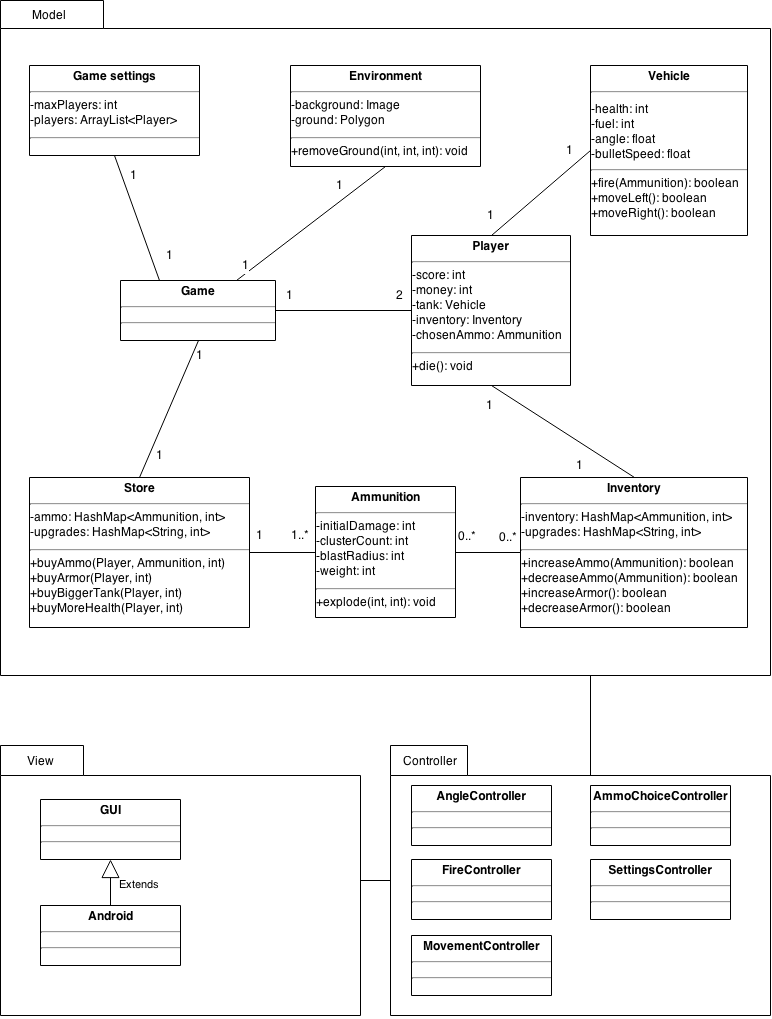
\includegraphics[scale=0.4]{images/logic_view.png}
\caption{Logic view}
\label{fig:logic-view}
\end{figure}

Our logic view (see Figure \ref{fig:logic-view}) is based on the logic view from The “4+1” View Model of Software Architecture \cite{krutchen}, but was built with a more recent modeling tool, UML. The modelling is also influenced by examples using the MVC-pattern from the lectures.

The logic view has been separated the different classes into the different parts of MVC. The model contains the classes which hold information about the game, such as game settings and players. These classes are specified with their most important fields and methods, e. g. a vehicle’s ability to fire or the initial damage of a certain ammunition type. It also covers the relationship between the classes, specifying which classes are connected and how many of these relations are allowed.
The controller simply contains the different controllers which will be used to change values in the model, based on what the user does in the view (GUI).
The view contains a GUI- and an Android-class, to illustrate that the view mainly consists of a GUI and that we wish to implement this GUI on a device running the Android OS. Implementing the GUI will be made easier by using the framework libGDX, but this is not shown in the view part, as libGDX will be utilized for other operations as well (e. g. game logic). 

As previously mentioned, we want to use libGDX to ease development. We have not included this in the logic view, as the full extent to which we will utilize libGDX is not decided, due to inexperience with the framework. 


\section{Process View}
\begin{figure}
\centering
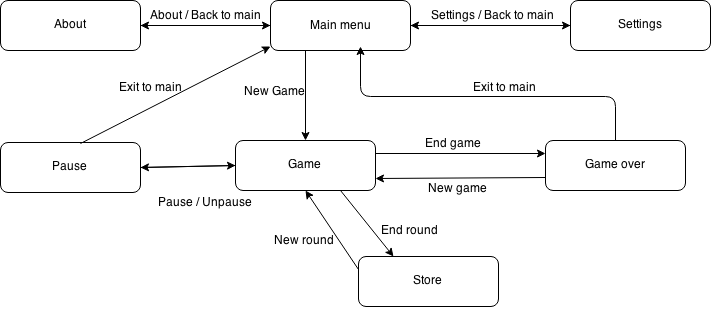
\includegraphics[scale=0.4]{images/process_view.png}
\caption{Process view}
\label{fig:process-view}
\end{figure}

Figure \ref{fig:process-view} shows the process view of the application. It is divided into the different scenes you will encounter when playing the game. You start at the “Main menu”. 

The double arrows symbolizes a splash screen that will be put on top of the scene you came from (e.g. when going from “Main menu” to “Settings”, the “Settings” scene will be put on top of “Main menu” and removed when abandoned.). A single arrow will remove the current scene and generate the subsequent.

When starting the game, you have a couple of choices: you can get information about the game (“how to play” and who developed it), change the settings or start a game with predefined settings. When playing the game, you can pause the game and from there end it. When a round is over, you will be presented with the store, where you can buy upgrades and ammunition. When this is done, you will start a new round. When the game is over (i.e. a player has won) you will be presented with two choices: you can either start a new game with the same settings, or you can exit the game and go to the main menu.


\section{Developement View}

\begin{figure}
\centering
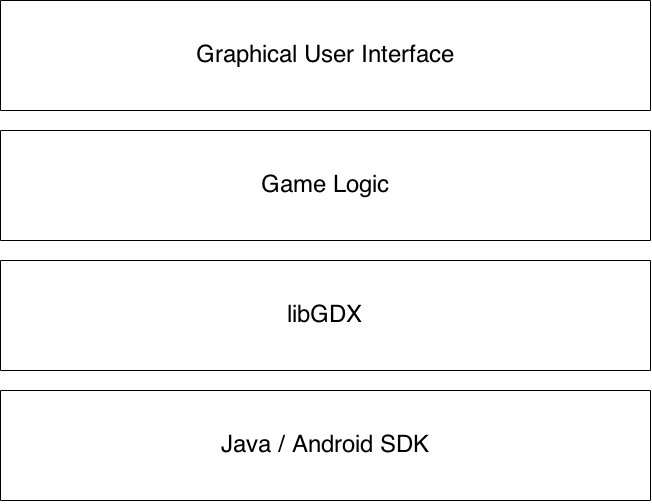
\includegraphics[scale=0.4]{images/development_view.png}
\caption{Development view}
\label{fig:development-view}
\end{figure}

The project is written in Java using the Android SDK. libGDX is the framework chosen for the game programming. These two gives us the foundation for writing our game logic and the game logic is used when writing the GUI. See Figure \ref{fig:development-view}.

\chapter{Consistency Among Views}
There are no inconsistencies among the views of our architecture. The views do not contradict one another. In addition, our views are contained in each other. Process View is contained in Logic View; the Logic View is contained in Development View.
\chapter{Architectural Rationale}
We have chosen the Model View Controller as our architectural pattern. The MVC pattern separates the data from the display, which allows each to change without the other changing. This increases our primary focus attribute, modifiability, because it keeps the various pieces separate and easy to modify independently. The pattern also enhances or secondary focus attribute; testability. It naturally separates different application concerns into different, independent software pieces, which makes unit testing of the individual pieces a lot easier.

As for design patterns, we want to use the Singleton Pattern. This is a good way to store the game settings, since they will be used across multiple components. A drawback with this pattern is that it may make the game less testable. Therefore we will only use this pattern in a limited way.
\chapter{Issues}
In this chapter, you should discuss the results you have obtained from your implementation.
These can be correctness results, i.e whether the implementation behaved as expected, or numerical results that express runtime or energy measurements.
\chapter{Changes}
In this chapter, you should discuss the results you have obtained from your implementation.
These can be correctness results, i.e whether the implementation behaved as expected, or numerical results that express runtime or energy measurements.

% Bibliography - edit references.bib and use the \cite command in text
\bibliographystyle{plain}
\bibliography{references}
\end{document}
